\chapter{Identification des facteurs influençant l'efficacité du Neurofeedback}

\section*{Introduction}

La réplication et la mise à jour de la méta-analyse de \citet{Cortese2016} décrite dans le chapitre précédent a permis de mettre en évidence la forte hétérogénéité des études incluses dans ce type d'analyse. 
En effet, même si ces études satisfont toutes le critère d'inclusion défini par les auteurs, elles diffèrent d'un point de vue technique et méthodologique : elles ont été rassemblées 
sans tenir compte par exemple de la qualité de l'acquisition de l'\gls{eeg}, du neuromarqueur entrainé lors du \gls{nfb} et du design de l'étude clinique (notamment le nombre de 
sessions et la durée du traitement). 

Afin de pallier ces limitations, une nouvelle approche a été implémentée : l'analyse systématique des biais (\gls{saob} en anglais) qui va justement tirer avantage de cette hétérogénéité. L'efficacité du traitement, quantifiée 
par l'\gls{es}-intra-groupe, de chaque intervention est considérée comme variable dépendante expliquée par des variables indépendantes qui sont ici les facteurs méthologiques et techniques. 
Le but de cette analyse est de déterminer les facteurs qui ont une influence sur l'efficacité du \gls{nfb} : au vu des résultats des précédentes méta-analyses \citep{Micoulaud2014, Cortese2016}, 
on peut notamment s'attendre à ce que les évaluateurs aveugles soient associés à une plus faible efficacité du traitement. 

\section{Extraction et pré-traitement des facteurs}

La première étape de la \gls{saob} est d'obtenir les facteurs des études sélectionnées. Une liste de facteurs ayant potentiellement une influence sur l'efficacité du \gls{nfb} a été 
établie, puis les facteurs ont été extraits de chaque étude. Avant de débuter l'analyse, les facteurs sont pré-traités en suivant les étapes décrites dans cette section. 

\subsection{Choix des facteurs}

Les facteurs ayant une possible influence sur l'efficacité du \gls{nfb} ont été répartis en cinq catégories :
\renewcommand{\labelitemi}{$\bullet$}
\begin{itemize}
\item \emph{les biais méthodologiques :} la présence d'un groupe contrôle, l'aveugle des évaluateurs (\gls{pblind}), la randomisation des sujets dans les essais contrôlés, et la validation de l'étude 
par un \gls{irb},
\item \emph{la population :} la prise de psychostimulants durant le traitement par \gls{nfb}, la tranche d'âge des enfants inclus, la sévérité des symptômes du TDAH à pré-test (score clinique à pré-test
divisé par le score maximal à atteindre sur l'échelle clinique), et le degré d'engagement dans l'entrainement par \gls{nfb},
\item \emph{l'implémentation du \gls{nfb} :} le protocole utilisé (\gls{scp}, \gls{smr}, l'augmentation du rythme theta, l'augmentation du rythme beta dans les aires centrales ou frontales 
et la diminution du rythme theta), la présence d'une phase de transfert lors de l'entrainenement par \gls{nfb}, l'utilisation d'une carte de transfert pour s'entrainer à la maison ou à l'école, 
le type de seuillage pour les récompenses discrètes, le nombre de sessions de \gls{nfb}, la durée et la fréquence des sessions, la durée du traitement, l'individualisation des bandes de fréquence
basée sur l'\gls{iapf}, et le couplage du \gls{nfb} avec l'\gls{emg}-Biofeedback.
\item \emph{la qualité de l'acquisition :} la présence de plus d'une électrode active et la qualité de l'\gls{eeg}. Cette dernière est représentée par un indicateur allant de 1 à 3, calculé sur les critères 
suivants : 
\begin{description} 
\item[le type d'électrode utilisée :] \gls{agcl}/Gel ou \gls{au}/Gel,
\item[le contrôle de l'impédance :] la vérification du bon contact entre la peau et les électrodes en gardant l'impédance inférieure à $40$k$\Omega$,
\item[la certification du matériel hardware utilisé :] le matériel doit être conforme à la norme ISO-60601-2-26 \citep{ISO}.
\end{description}

Un score de qualité de 3 est donné si tous les critères ci-dessus sont remplis. Si au moins l'un d'eux est satisfait, le score est de 2, sinon il est mis à 1.

\item \emph{la qualité du signal} : le rejet en temps réel (l'\textit{epoch} est exlu, pas de retour calculé) ou la correction (retour calculé sur l'\textit{epoch} débruité) des 
artefacts oculaires (\gls{eog}) et le rejet en temps réel d'artefacts génériques détectés grâce à leur large amplitude. 
\end{itemize}

Afin d'éviter tout biais, le nom des facteurs a été caché durant les analyses : il n'a été révélé que lorsque le modèle a été considéré comme valide notamment au niveau 
de la normalisation des variables et de la validation des hypothèses du modèle.  

\subsection{Pré-traitement des facteurs}

Les auteurs des études incluses dans la \gls{saob} ne précisent pas systématiquement toutes les valeurs des facteurs, ce qui conduit à des observations manquantes. Afin que 
les facteurs pour lesquels peu d'observations sont diponibles ne faussent pas l'analyse, un critère d'exclusion arbitraire a été mis en place : si pour un facteur le nombre d'observations 
manquantes excède plus de 20\% du nombre total d'observations, ce facteur est exclu. Les facteurs qui sont des variables catégorielles et qui
comportent quelques observations manquantes voient ces valeurs imputées et remplacées par -1.

Par ailleurs, comme cette analyse tire avantage de l'hétérogénéité des études, si un facteur a plus de 80\% d'observations identiques, celui-ci est également exclu. 

Il est important de noter qu'une étude ne correspond pas nécessairement à une observation : lorsque plusieurs échelles cliniques et/ou évaluateurs sont disponibles dans une étude,
chaque couple échelle clinique-évaluateur est considéré comme une observation.

Ensuite, les facteurs qui sont des variables catégorielles (le protocole utilisé par exemple) sont codés en \textit{dummies} : la présence du facteur est représentée par un 1 et son absence par 0. 

Enfin, toutes les variables sont standardisées : à chaque observation est soustraite la moyenne de l'ensemble des observations, le tout divisé par l'écart-type de la moyenne de 
l'ensemble des observations. 

Les facteurs sélectionnés et prétraités sont les variables indépendantes de l'analyse.


\section{Explication de l'efficacité du Neurofeedback par des méthodes multivariées}

\subsection{Calcul de la taille d'effet intra-groupe}

L'\gls{es}-intra-groupe est calculé à partir des moyennes et écart-types des scores cliniques totaux donnés par les parents et les enseignants. De plus, lorsqu'une étude 
fournit des résultats pour plus d'une échelle clinique, l'\gls{es}-intra-groupe est calculé pour chaque échelle :
\begin{equation}
\label{eq:factors_effect_size_within_subject}
\text{ES-intra-groupe} = \frac{M_{\text{post},T} - M_{\text{pré},T}}{\sqrt{\frac{\sigma_{\text{pré},T}^2 + \sigma_{\text{post},T}^2}{2}}},
\end{equation} 
\noindent où $M_{\text{t},T}$ est la moyenne sur l'échelle clinique, pour le traitement $T$, au moment t (pré-test ou post-test) et $\sigma_{\text{t},T}$ représente
son écart-type. Au contraire de l'\gls{es}-inter-groupes défini à l'équation Eq.~(\ref{eq:metareview_effect_size_between}), cet \gls{es} permet de se concentrer sur l'effet du 
traitement au sein du groupe \citep{Cohen1988}. Cette définition de l'\gls{es} a déjà été précédemment utilisée dans la littérature sur le \gls{nfb} 
appliquée aux enfants \gls{tdah} \citep{Arns2009, Maurizio2014, Strehl2017}. 

Enfin, afin d'éviter de rompre les hypothèses des méthodes utilisées dans la \gls{saob}, les valeurs non comprises dans l'intervalle 
$[\mu - 3 \sigma, \mu + 3 \sigma]$ (avec $\mu$ et $\sigma$ respectivement la moyenne et l'écart-type de tous les \gls{es}-intra-groupe calculés \citep{Shewhart1931})
sont considérées comme aberrantes et sont donc rejetées.

Par la suite, l'ensemble des \gls{es}-intra-groupe est considéré comme la variable dépendante que les variables indépendantes (les facteurs) vont expliquer. 

\subsection{L'analyse systématique des biais}

La \gls{saob} comporte trois méthodes qui ont été implémentées à l'aide des bibliothèques Python Scikit-Learn \citep[version 0.18.1]{Pedregosa2011} et Statsmodels \citep[version 0.8.0]{Seabold2010} : 
\begin{itemize}
  \item Une régression linéaire multiple et pondérée (\gls{wls} en anglais) \citep{Montgomery2012},
	\item Une régression linéaire régularisée (\gls{lasso} en anglais) \citep{Tibshirani1996},
	\item Un arbre de décision de regression (\gls{dt} en anglais) \citep{Quinlan1986}.
\end{itemize}

\subsubsection{La régression linéaire multiple et pondérée}
La régression linéaire a pour but d'estimer les coefficients de régression qui lient les facteurs aux \gls{es}-intra-groupe. Ici, la régression est pondérée pour, d'une part, 
prendre en compte le fait que pour certaines études plusieurs échelles cliniques sont disponibles, et d'autre part pour capturer les différentes tailles d'échantillon parmi les études.
Le poids $w_{n}$ associé à chaque observation $n$ est défini comme suit : 
\begin{equation}
\label{eq:weight_WLS}
w_{n} = \frac{\text{N}_{k,T}}{\text{NScales}_{k,T}},
\end{equation} 
avec $\text{N}_{k,T}$ le nombre de sujets dans l'étude $k$ dans le groupe suivant le traitement $T$ et $\text{NScales}_{k,T}$ le nombre 
d'échelles cliniques disponibles dans l'étude $k$ évaluant l'efficacité du traitement $T$.

Mathématiquement, la \gls{wls} se traduit ainsi : 
\begin{equation}
\label{eq:factors_model_WLS}
\textbf{W}y = \textbf{WX}\beta + \epsilon.
\end{equation}
$\textbf{X}$ est une matrice inversible $(n \times p)$ et représente $n$ observations sur chaque $p-1$ variable indépendante et l'intercept, 
$\beta$ est un vecteur $(p \times 1)$ des coefficients de régression associés, $\textbf{W}$ est une matrice diagonale $(n \times n)$  
des poids $w_{n}$, $y$ est un vecteur $(n \times 1)$ des variables dépendantes et $\epsilon$ est un vecteur $(n \times 1)$ d'erreurs.

Le but de la \gls{wls} est d'estimer le vecteur de coefficients $\beta$ en minimisant la somme pondérée des carrés des résidus (\gls{wrss} en anglais) :
\begin{equation}
\label{eq:factors_WRSS}
\text{WRSS} = \sum_{i=1}^{n} w_i \Big(y_i - \beta_{0} - \sum_{j=1}^{p}\beta_{j}x_{ij}\Big)^2.
\end{equation}

Une fois le vecteur $\beta$ estimé, on cherche à savoir si les hypothèses du modèle sont vérifiées : 
\begin{itemize}
	\item la matrice ${\textbf{X}}^{T}\textbf{W}^{T}\textbf{WX}$ est régulière,
  \item aucune corrélation apparente n'est trouvée entre les variables indépendantes non catégorielles, 
  \item la tendance linéaire estimée est trouvée significative en se basant sur la statistique F,
  \item les résidus sont distribués normalement en se basant sur le kurtosis et le test Omnibus.
\end{itemize} 

Si toutes ces hypothèses sont satisfaites, on peut interpréter les résultats de la \gls{wls}. On s'intéresse à la significativité de chaque coefficient $\beta_{j, 1<j<p}$ :
s'il est significatif, le facteur associé à ce coefficient est supposé avoir une influence sur l'efficacité du \gls{nfb}. Par ailleurs, le signe du coefficient indique si 
cette influence est positive ou négative. 

Etant donné le nombre important de vraiables indépendantes, le pourcentage de variance estimée par la \gls{wls} est par le coefficient de détermination ajusté 
(\textit{adjusted R-Squared} en anglais) plutôt que par le coefficient de détermination (\textit{R-Squared} en anglais).

Une régression linéaire ordinaire (\gls{ols} en anglais) est aussi mise en place pour observer l'impact des poids sur les résultats. 

\subsubsection{La régression linéaire régularisée}

La deuxième méthode appliquée lors de la \gls{saob} est le \gls{lasso} qui intègre la sélection de variables dans le modèle linéaire grâce à la norme $\ell_1$ appliquée aux coefficients.
Les coefficients $\hat{\beta}_{j, 1<j<p}$ sont obtenus en minimisant le coût :
\begin{equation}
\label{eq:factors_lasso-minimization}
\hat{\beta} = \argmin_\beta \sum_{i=1}^{n} \Big(y_i - \beta_{0} - \sum_{j=1}^{p}\beta_{j}x_{ij}\Big)^2 + \lambda \sum_{j=1}^{p}\abs{\beta_{j}},
\end{equation} 
où $\lambda$ est le paramètre de régularisation qui, en augmentant, met de plus en plus de coefficients à 0. 

Le paramètre de régularisation optimal est déterminé par une validation croisée \textit{leave-one-out}. Cette méthode prend une seule observation 
comme donnée de test pour la validation, laissant $n$ - 1 observations pour les données d'entraînement. Le processus de la validation croisée est ensuite répété $n$ fois pour que chaque observation 
soit utilisée exactement une fois comme donnée de test. Pour chaque itération, appelée \textit{fold} en anglais, l'erreur quadratique moyenne (\gls{mse} en anglais) est calculée sur les données de test
puis les $n$ resultats sont moyennés pour mener à une seule observation qui permet de trouver le $\lambda$ optimal. Celui-ci correspond à l'abscisse du minimum de la \gls{mse} 
du \textit{fold} moyen calculée sur un large intervalle de $\lambda$ \citep{James2013}.
Un coefficient non mis à 0 signifie que le facteur associé pourrait avoir une influence sur l'efficacité du \gls{nfb} et, ici aussi, le signe du coefficient indique la direction de l'effet. 

\subsubsection{L'arbre de décision de régression}

La troisième et dernière méthode utilisée est le \gls{dt} de régression qui, à l'inverse des deux précédentes méthodes, n'est pas une méthode 
linéaire \citep{Quinlan1986}. Elle divise l'ensemble des observations en sous-ensembles de plus en plus petits en se basant sur la présence 
d'une variable qualitative ou sur la comparaison à un seuil appliqué à une variable quantitative. La position de la variable indépendante utilisée (et le
seuil de comparaison dans le cas d'une variable quantitative) pour subdiviser l'ensemble des données est déterminée de façon à minimiser la
\gls{mse} définie comme suit :

\begin{equation}
\label{eq:factors_decision_tree_mse}
\text{MSE} = \frac{1}{n}\sum_{i=1}^{n} \Big(\hat{y}_i - {y}_i\Big)^2,
\end{equation}
avec $\hat{y}$ les valeurs prédites.

La première variable utilisée pour diviser l'ensemble des données se situe dans le noeud racine (\textit{root node} en anglais), les autres
variables qui mènent à une nouvelle subdivision sont dans des noeuds, et les noeuds où la divsion s'arrête sont appelés
feuilles (\textit{leaf nodes}) de l'arbre. La profondeur de l'arbre peut être définie par le nombre d'observations minimal nécessaire
pour diviser un sous ensemble. Un arbre exemple est schématisé à la Figure~\ref{Figure:factors_decision_tree_example}.

\begin{figure}[h!]
  \centering
	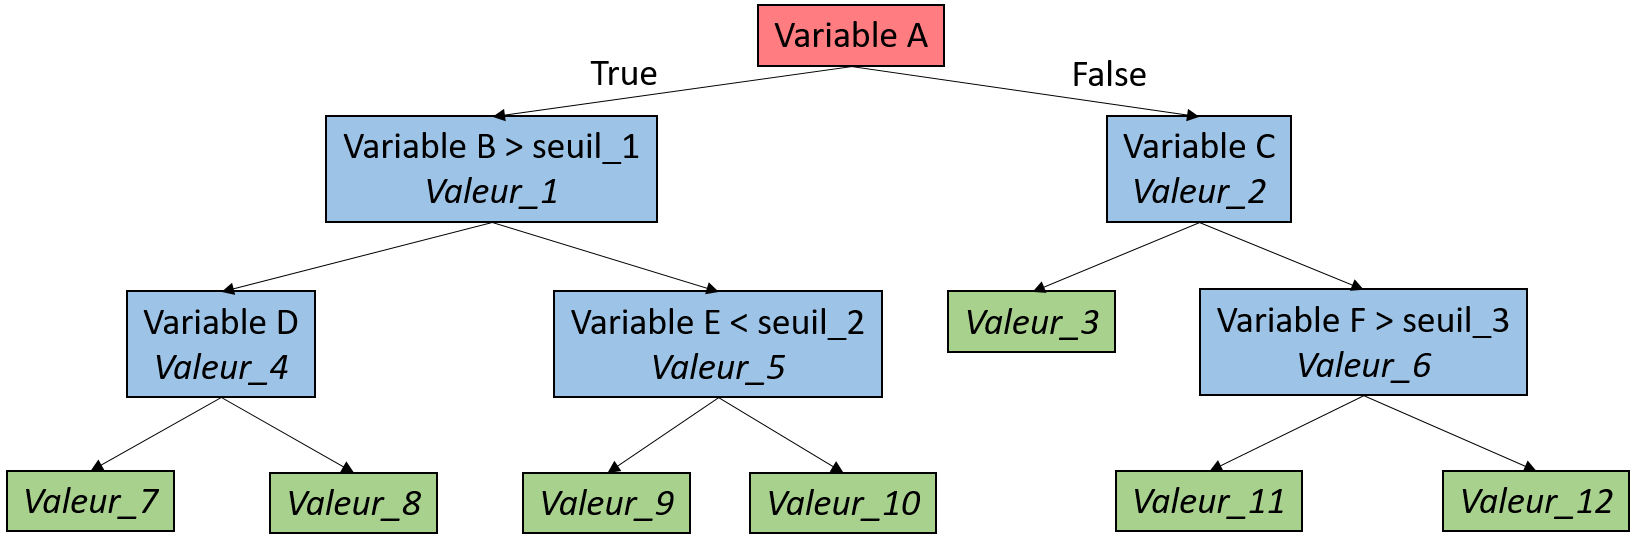
\includegraphics[width=1.0\linewidth]{figures/chapter-3/decision-tree-example} 
  \caption{Exemple schématique d'arbre de décision de régression. Le \textit{root node} est en rouge, les noeuds sont en bleu et les feuilles en vert. 
	Les variables A, C et D sont catégorielles ; les variables B, E et F sont numériques. Les valeurs dans les feuilles correspondent à la valeur 
	prédite par l'arbre de décision de la variable dépendante.}
  \label{Figure:factors_decision_tree_example}
\end{figure}

Cette méthode gère facilement les valeurs manquantes : ainsi aucune imputation n'a été effectuée avant le calcul du \gls{dt}. Dans le cas de la \gls{saob}, 
les facteurs se retrouvent dans les feuilles : leur influence sur l'efficacité du \gls{nfb} est quantifiée par la valeur de la variable dépendante 
obtenue après chaque division mais aussi par leur place dans l'arbre. En effet, plus un facteur est en haut de l'arbre plus les divisions se font sur un grand nombre
d'observations, ainsi son impact sur l'efficacité a plus de chance d'être avérée.

\section{Analyse des facteurs influençant le Neurofeedback}

\subsection{Sélection des études}

Les termes entrés dans Pubmed pour la recherche des articles à inclure dans la \gls{saob} sont :
(ADHD OR adhd OR attention deficit disorder with hyperactivity OR minimal brain disorders OR syndrome hyperkinetic OR hyperkinetic
 syndrome OR hyperactivity disorder OR hyperactive child syndrome OR childhood hyperkinetic syndrome OR attention deficit hyperactivity disorders
 OR attention deficit hyperactivity disorder OR adhd attention deficit hyperactivity disorder OR addh OR overactive child syndrome OR attention deficit 
hyperkinetic disorder OR hyperkinetic disorder OR attention deficit disorder hyperactivity OR attention deficit disorders hyperactivity OR child 
attention deficit disorder OR hyperkinetic syndromes OR syndromes hyperkinetic OR hyperkinetic syndrome childhood) AND 
(randomized control trial OR RCT OR randomized control study OR Pilot Study OR Study OR Trial OR randomized trial) AND 
(neurofeedback OR “EEG biofeedback” OR neurotherapy OR SCP OR “slow cortical potentials” OR Theta Beta Ratio OR “TBR”). 

La dernière recherche effectuée le 12 février 2018 avec ces termes a retourné 155 résultats, auxquels se sont ajoutés 22 articles inclus dans les précédentes 
méta-analyses sur le \gls{nfb} appliqué aux enfants \gls{tdah} \citep{Arns2009, Sonuga-Barke2013, Micoulaud2014, Cortese2016, Catala2017}. Afin de sélectionner
les études à inclure dans la \gls{saob}, les 177 résultats ont été filtrés à l'aide d'un pipeline représenté à la 
Figure~\ref{Figure:factors_pipeline_selection_studies}. Au final $k$ = 33 études ont été sélectionnées, qui correspondent par ailleurs au critère d'inclusion de
\citet{Cortese2016} sans les exigences sur les groupes contrôles. 

\newpage\
\begin{figure}[h!]
  \centering
	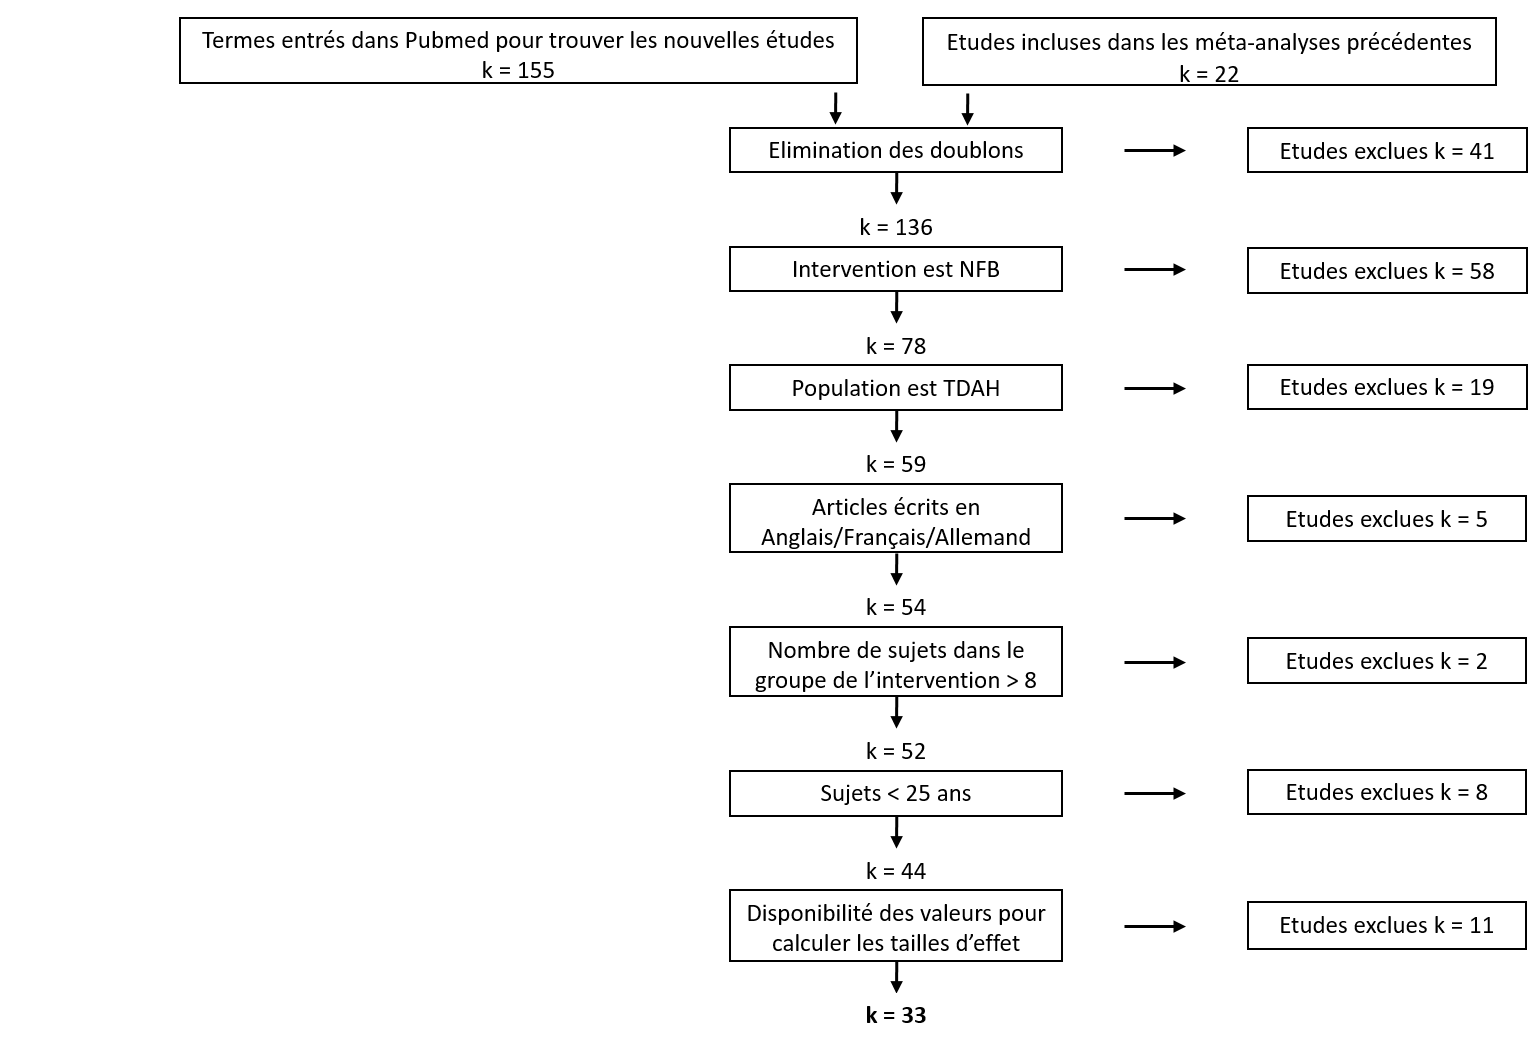
\includegraphics[width=1.0\linewidth]{figures/chapter-3/factors-selection-studies} 
  \caption{Diagramme de sélection des études pour l'analyse systématique des biais (dernière recherche le 12 fevrier 2018).}
  \label{Figure:factors_pipeline_selection_studies}
\end{figure}

Les \gls{es}-intra-groupe sont calculés pour chaque étude puis les valeurs aberrantes sont rejetées. La distribution des \gls{es}-intra-groupe ainsi que les bornes 
de l'intervalle d'inclusion sont représentés à la Figure~\ref{Figure:distribution_ES_within}. Les \gls{es}-intra-groupe négatifs sont en faveur du \gls{nfb}.

\begin{figure}[h!]
  \centering
	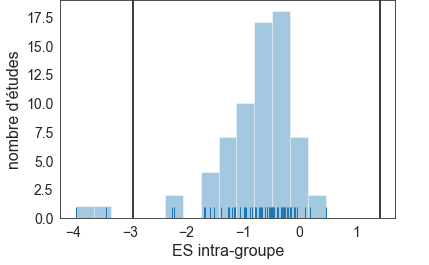
\includegraphics[width=0.7\linewidth]{figures/chapter-3/distribution-ES-within} 
  \caption{Distribution des tailles d'effet (\gls{es}) intra-groupe, une valeur négative est en faveur du Neurofeedback. Les lignes verticales noires correspondent aux bornes supérieure et 
	inférieure de l'intervalle dans lequel les observations sont acceptées.}
  \label{Figure:distribution_ES_within}
\end{figure}

Deux observations sont à l'extérieur de l'intervalle d'inclusion : deux groupes de sujets de \citet{Bazanova2018} (celui de l'individualisation du \gls{nfb} et celui de
l'individualisation du \gls{nfb} et du couplage avec \gls{emg}-Biofeedback). En effet, ces deux groupes présentent des \gls{es}-intra-groupe très larges (respectivement -3.41 et -3.95)
qui sont même plus élevés que ceux reportés dans la littérature sur l'efficacité des psychostimulants sur les symptômes du \gls{tdah} chez les enfants \gls{tdah} \citep{Luan2017}.
Ces valeurs invalident nos hypothèses de travail, ainsi afin de pouvoir conclure sur les résultats obtenus par la \gls{saob}, un rejet des valeurs aberrantes a été implémenté.

La \gls{saob} est donc effectuée sur 33 études (qui correspondent à 67 observations) évaluant l'efficacité du \gls{nfb} sur les enfants \gls{tdah} et qui son listées dans la 
Table~\ref{Table:table_factors_analysis_meta_analysis_list_studies}. Au total, les 33 études sélectionnées rassemblent 846 enfants \gls{tdah} effectuant du \gls{nfb}.

\newpage\
\begin{table}[h!]
  \centering
  \caption{Liste des études incluses dans l'analyse systématique des biais : a) études incluses dans \citet{Cortese2016}
	(dernière recherche le 30 août 2015) ; b) études satisfaisant le critère d'inclusion de \citet{Cortese2016} (dernière recherche le 12 février 2018) ; c) études 
	satisfaisant le critère d'inclusion de \citet{Cortese2016} à l'exception de la partie concernant le groupe contrôle (dernière recherche le 12 février 2018).}
  \fontsize{9}{11}\selectfont
\begin{tabular}{ cccccc }
\toprule
\multicolumn{3}{ c }{Analyse} & Etude & Année & \shortstack{ Nombre de sujets \\ dans le groupe \\ \gls{nfb} } \\
\midrule
 & & & \citeauthor{Arnold2014} & 2014 & 26 \\ 
 & & & \citeauthor{Bakhshayesh2011} & 2011 & 18 \\
 & & & \citeauthor{Beauregard2006} & 2006 & 15 \\
 & & & \citeauthor{Bink2014} & 2014 & 45 \\
 & & & \citeauthor{Christiansen2014} & 2014 & 14 \\
 & & & \citeauthor{Gevensleben2009} & 2009 & 59 \\
 & & & \citeauthor{Heinrich2004} & 2004 & 13 \\
 & & & \citeauthor{Holtmann2009} & 2009 & 20 \\
 & & & \citeauthor{Linden1996} & 1996 & 9 \\
 & & & \citeauthor{Maurizio2014} & 2014 & 13 \\
 & & & \citeauthor{Steiner2011} & 2011 & 9 \\
 & & & \citeauthor{Steiner2014} & 2014 & 34 \\
 & & & \citeauthor{VanDongen2013} & 2013 & 22 \\
 & & \shortstack{a = Réplication de \\ \citeauthor{Cortese2016}  \\ (voir \ref{replication}) } & \textbf{13 études} & & \textbf{297} \\
\cmidrule(lr){3-6}
 & & & \citeauthor{Aggensteiner2019} & 2019 & 75 \\
 & & & \citeauthor{Baumeister2016} & 2016 & 8 \\
 & & & \citeauthor{Bazanova2018} & 2018 & 17 \\
 & & & \citeauthor{Minder2018} & 2018 & 38 \\
 & & & \citeauthor{Moreno2019} & 2019 & 19 \\
 & & & \citeauthor{Strehl2017} & 2017 & 72 \\
 & & & \citeauthor{Shereena2019} & 2019 & 15 \\
 & \shortstack{b = Mise à jour \\ \citeauthor{Cortese2016} \\ (voir \ref{selection_studies}) } & & \textbf{16 études} & & \textbf{541} \\
\cmidrule(lr){2-6}
 & & & \citeauthor{Bluschke2016} & 2016 & 19 \\
 & & & \citeauthor{Cueli2019} & 2019 & 64 \\
 & & & \citeauthor{Deilami2016} & 2016 & 12 \\
 & & & \citeauthor{Drechsler2007} & 2007 & 17 \\
 & & & \citeauthor{Duric2012} & 2012 & 23 \\
 & & & \citeauthor{Escolano2014} & 2014 & 20 \\
 & & & \citeauthor{Fuchs2003} & 2003 & 22 \\
 & & & \citeauthor{Gelade2016} & 2016 & 39 \\
 & & & \citeauthor{Heinrich2019} & 2019 & 60 \\
 & & & \citeauthor{Kropotov2005} & 2005 & 86 \\
 & & & \citeauthor{Lee2017} & 2017 & 18 \\
 & & & \citeauthor{Leins2007} & 2007 & 19 \\
 & & & \citeauthor{Li2013} & 2013 & 32 \\
 & & & \citeauthor{Meisel2014} & 2014 & 12 \\
 & & & \citeauthor{Mohagheghi2017} & 2017 & 30 \\
 & & & \citeauthor{Mohammadi2015} & 2015 & 16 \\
 & & & \citeauthor{Monastra2002} & 2002 & 51 \\
 & & & \citeauthor{Ogrim2013} & 2013 & 13 \\
 & & & \citeauthor{Rajabi2019} & 2019 & 16 \\
 & & & \citeauthor{Sudnawa2018} & 2018 & 20 \\
 & & & \citeauthor{Strehl2006} & 2006 & 23 \\
 c = \gls{saob} & & & \textbf{41 études} & & \textbf{1 153} \\
\bottomrule
\end{tabular}

  \label{Table:table_factors_analysis_meta_analysis_list_studies}
\end{table}

\newpage\
\subsection{Facteurs identifiés}

Vingt-huit facteurs ont été initialement identifiés afin d'analyser leur influence sur l'efficacité du \gls{nfb}. Parmi ces facteurs, neuf ont dû être exclus car ils étaient trop
homogènes ou présentaient trop d'observations manquantes : 
\begin{itemize}
	\item l'augmentation du rythme beta dans les aires frontales,
  \item l'utilisation d'une carte pour le transfert de l'entrainement à la maison et à l'école, 
  \item le type de seuillage pour les récompenses discrètes (incrémental ou fixe),
  \item la qualité de l'acquisition de l'\gls{eeg} égale à 3,
	\item la présence d'un groupe contrôle,
	\item l'individualisation des bandes de fréquences basée sur la valeur de l'\gls{iapf},
	\item le couplage entre le \gls{nfb} et l'\gls{emg}-Biofeedback,
	\item la sévérité des symptômes du \gls{tdah},
	\item le degré d'engagement dans l'entraînement par \gls{nfb}.
\end{itemize} 

Les trois méthodes décrites précédemment sont donc appliquées tour à tour sur les 19 facteurs restants. Tous les résultats sont résumés dans la Table~\ref{Table:table_factors_analysis_results_summary}.

\newpage\
\begin{table}[h!]
  \centering
  \caption{Resultats de la régression linéaire pondérée (\gls{wls}), de la régression linéaire régularisée (\gls{lasso}) et de l'arbre de décision (\gls{dt}). Pour la \gls{wls}, une p-value $<$ 0.05 
	(en gras) signifie que le coefficient du facteur correspondant est significativement différent de 0. Pour le \gls{lasso}, les facteurs dont les coefficients sont non mis à 0 (en gras) sont 
	sélectionnés. Pour l'arbre de décision, la place du facteur dans l'arbre est indiquée. Pour les deux premières colonnes, quand la valeur du coefficient est négative le facteur 
	correspondant pourrait mener à de meilleurs résultats du \gls{nfb}.}
  \begin{center}
\small 
\begin{tabular}{ p{3cm} p{3cm} p{3cm} p{2cm} p{2cm} p{2cm}}
\toprule
\multicolumn{2}{c}{ \shortstack{Variables \\ indépendantes (facteurs)} } & \shortstack{ Coefficients \\ trouvés par \gls{wls} \\ ($p$-value) } & \shortstack{ Coefficients \\ trouvés par \\ \gls{lasso} } & \shortstack{Place \\ sur le \\ \gls{dt}} \\
\midrule
\multirow{ 3}{*}{ \textit{Méthodologiques} } & \gls{pblind} & \hskip 0.12in\textbf{0.15 (0.015)} & \hskip 0.12in\textbf{0.086} & \textbf{\textit{root node}} \\ 
& randomisation & \hskip 0.12in0.013 (0.840) & \hskip 0.12in0.00 & / \\   
\midrule
\multirow{ 3}{*}{ \textit{Population} } & age max & \hskip 0.08in-0.10 (0.106) & \hskip 0.12in0.00 & / \\
& age min & \hskip 0.12in0.056 (0.43) & \hskip 0.12in0.00 & / \\
& prise de médicaments & \hskip 0.08in-0.026 (0.72) & \hskip 0.12in0.00 & / \\
\midrule
\multirow{ 9}{*}{ \textit{ \shortstack{Implementation \\ du \gls{nfb}} } } & nombre de sessions & \hskip 0.08in\textbf{-0.19 (0.025)} & \hskip 0.12in0.00 & / \\
& durée de la session & \hskip 0.08in-0.13 (0.16) & \hskip 0.12in0.00 & \textbf{2$^{eme}$ noeud} \\
& durée du traitement & \hskip 0.12in\textbf{0.39 (0.00)} & \hskip 0.12in\textbf{0.098} & \textbf{2$^{eme}$ et 3$^{eme}$ noeuds} \\
& fréquence des sessions & \hskip 0.12in0.027 (0.690) & \hskip 0.08in\textbf{-0.055} & \textbf{2$^{eme}$ noeud} \\ 
& \gls{smr} & \hskip 0.12in0.12 (0.067) & \hskip 0.12in0.00 & / \\
& augmentation de beta en central & \hskip 0.12in0.087 (0.32) & \hskip 0.12in\textbf{0.026} & / \\  
& diminution de theta & \hskip 0.08in-0.095 (0.39) & \hskip 0.12in0.00 & / \\
& \gls{scp} & \hskip 0.08in-0.14 (0.30) & \hskip 0.12in0.00 & / \\ 
& phase de transfert & \hskip 0.12in\textbf{0.33 (0.001)} & \hskip 0.12in\textbf{0.079} & \textbf{1$^{er}$ noeud} \\
\midrule
\multirow{ 2}{*}{ \textit{ \shortstack{Qualité de \\ l'acquisition} } } & plus d'une électrode d'enregistrement & \hskip 0.08in-0.083 (0.20) & \hskip 0.08in\textbf{-0.030} & / \\ 
& \gls{eeg} qualité 2 & \hskip 0.08in\textbf{-0.28 (0.00)} & \hskip 0.08in\textbf{-0.037} & / \\  
\midrule
\multirow{ 2}{*}{ \textit{Qualité du signal} } & rejet ou correction des artefacts oculaires & \hskip 0.08in-0.10 (0.164) & \hskip 0.08in\textbf{-0.0046} & \textbf{1$^{er}$ noeud} \\ 
& rejet des artefacts basé sur l'amplitude & \hskip 0.12in0.14 (0.058) & \hskip 0.12in0.00 & / \\   
\bottomrule
\end{tabular}
\end{center}

  \label{Table:table_factors_analysis_results_summary}
\end{table}

\subsubsection{La régression linéaire multiple et pondérée}

Les hypothèses de ce modèle sont respectées, les résultats sont interprétables :
\begin{itemize}
	\item la matrice ${\textbf{X}}^{T}\textbf{W}^{T}\textbf{WX}$ est bien régulière,
  \item aucune corrélation apparente n'est effectivement trouvée entre les variables indépendantes non catégorielles, 
  \item la tendance linéaire estimée est trouvée significative (Prob(F-statistic) = 7.58e-08),
  \item les résidus sont distribués normalement (kurtosis = 3.154 et Prob(Omnibus) = 0.392).
\end{itemize}

La \gls{wls} a trouvé 9 facteurs significatifs (deuxième colonne de Table~\ref{Table:table_factors_analysis_results_summary}) avec un \textit{adjusted R Squared} de 0.62. 
Dans le cas de l'\gls{ols}, les mêmes facteurs ont été trouvés significatifs (à l'exception de qualité de 
l'\gls{eeg} égal à 2 et la présence de plus d'une électrode active) mais avec un \textit{adjusted R Squared} plus faible (0.35). Un facteur 
dont le coefficient est négatif serait en faveur de l'efficacité du \gls{nfb}.


\subsubsection{La régression linéaire régularisée}

La validation croisée \textit{leave-one-out} illustrée à la Figure~\ref{Figure:selection_lambda_lasso} a permis de déterminer un $\lambda$ optimal égal à 0.059.
\begin{figure}[h!]
  \centering
	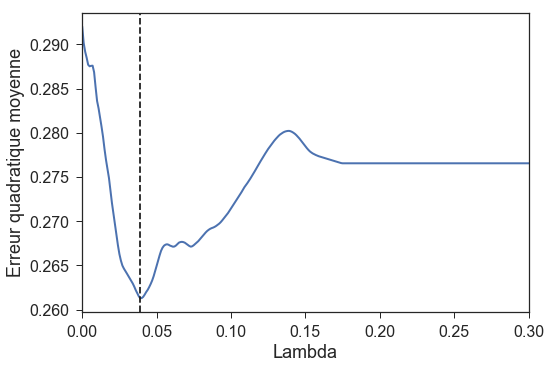
\includegraphics[width=0.7\linewidth]{figures/chapter-3/factors-selection-lasso-best-lambda} 
  \caption{Erreur quadratique moyenne obtenue sur la moyenne de tous les \textit{folds} utilisés lors de la validation croisée \textit{leave-one-out}.}
  \label{Figure:selection_lambda_lasso}
\end{figure}

Le \gls{lasso} a gardé six facteurs différents de 0 (troisième colonne de Table~\ref{Table:table_factors_analysis_results_summary}). Pour cette méthode également,
un facteur dont le coefficient est négatif aurait un bon impact sur l'efficacité du \gls{nfb}.

\subsubsection{L'arbre de décision de régression}

L'arbre de décision obtenu est présenté à la Figure~\ref{Figure:factors_decision_tree} : \gls{pblind} est le meilleur prédicteur (dernière colonne de 
Table~\ref{Table:table_factors_analysis_results_summary}). Quatre autres facteurs divisent ensuite les sous-ensembles, toutefois étant donné que de moins
en moins d'observations sont disponibles plus on descend dans l'arbre, l'influence de ces facteurs est de moins en moins certaine.

\begin{figure}[h!]
  \centering
	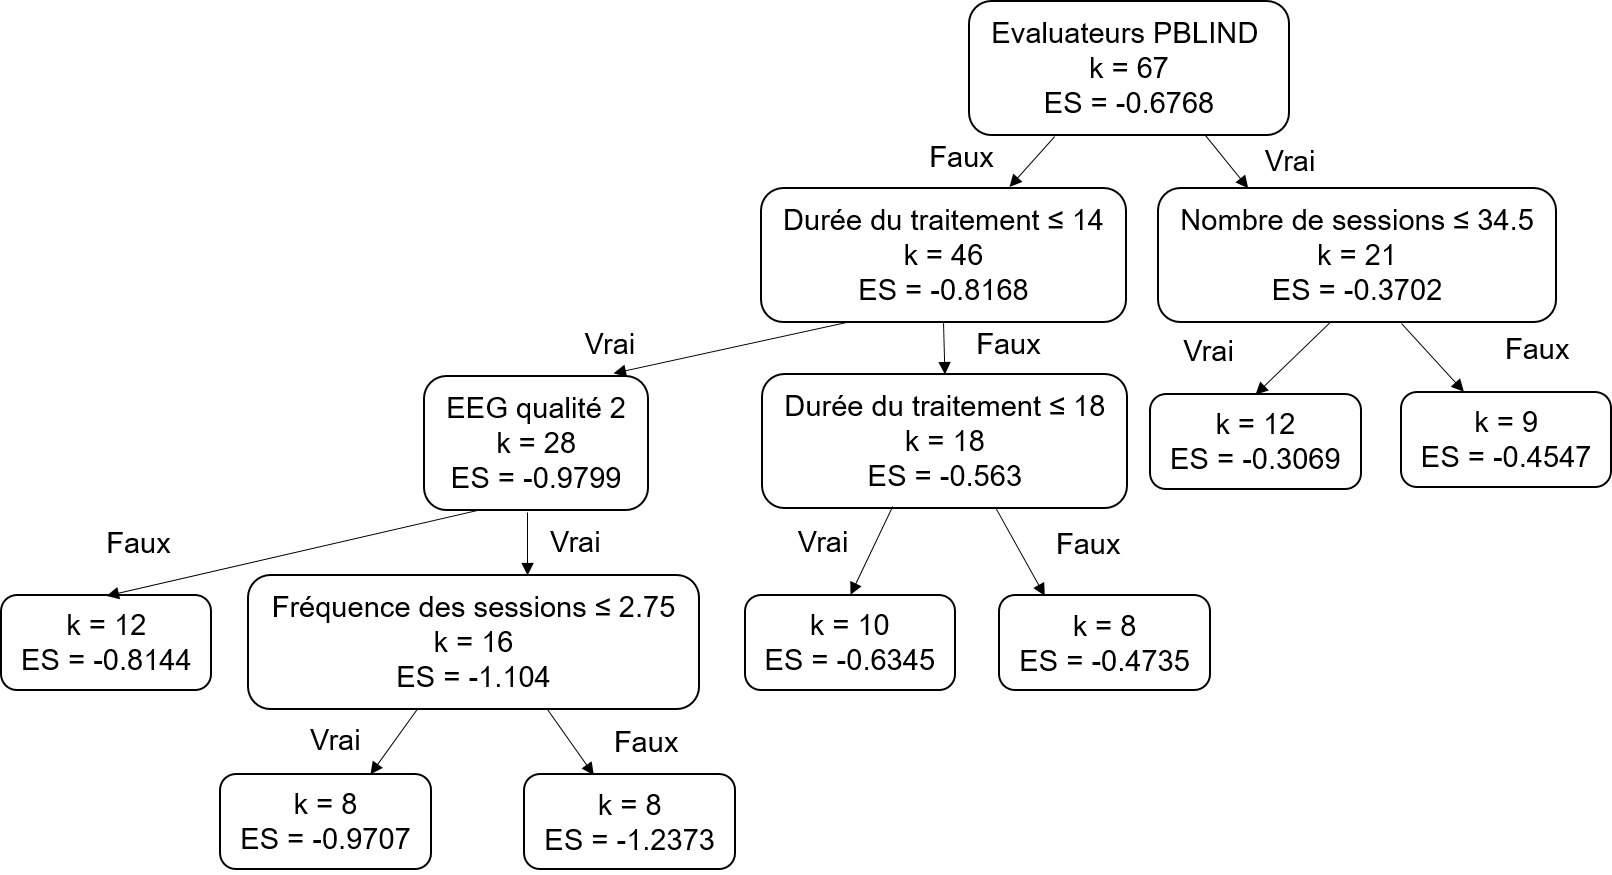
\includegraphics[width=1\linewidth]{figures/chapter-3/factors-decision-tree} 
  \caption{Arbre de décision obtenu : \gls{es} correspond à l'\gls{es}-intra-groupe et $k$ au nombre d'études. L'importance des variables indépendantes
	décroît depuis le \textit{root node}. La durée de la session est mesurée en minutes, la durée du traitement en semaines et l'âge en années.}
  \label{Figure:factors_decision_tree}
\end{figure}

\subsubsection{Résumé des résultats}

Plusieurs facteurs ont été trouvés significatifs par plusieurs méthodes, notamment les évaluateurs \gls{pblind}, la qualité de l'\gls{eeg} égale à 2 et la durée du traitement. 
De plus, dans le cas de ces trois facteurs, toutes les méthodes s'accordent quant à la direction de leur influence : alors qu'évaluer l'efficacité du \gls{nfb} en étant \gls{pblind}
semble conduire à de moins bons résultats, une durée de traitement plus courte et l'acquisition de l'\gls{eeg} avec un bon matériel mèneraient à un traitement plus efficace. 

L'influence des facteurs retournés par une ou deux méthodes est plus incertaine :
\begin{itemize}
	\item la \gls{wls} et le \gls{lasso} trouvent tous deux qu'utiliser plus d'une électrode active durant la session de \gls{nfb} mènerait à de bons résultats,
  \item la \gls{wls} et le \gls{dt} conluent tous deux qu'effectuer un grand nombre de sessions est préférable, 
  \item le \gls{lasso} et le \gls{dt} obtiennent tous deux qu'un nombre élevé de sessions par semaine influencerait positivement les résultats. 
\end{itemize}

Cinq facteurs sont retournés seulement par une méthode : la randomisation des groupes, le recours à un \gls{irb}, la durée de la session, la présence d'une phase de transfert,
et la correction ou rejet des artefacts oculaires. Huit facteurs, n'ont quant à eux été sélectionnés par aucune méthode : l'âge minimum et maximum des enfants, prendre des 
médicaments pendant le traitement par \gls{nfb}, les protocoles \gls{smr}, augmentation de beta dans les aires centrales, diminution de theta et \gls{scp}, et la correction
des artefacts basée sur l'amplitude. Ainsi ces facteurs n'influenceraient pas l'efficacité du \gls{nfb}. Par la suite, seuls les facteurs sélectionnés par au moins deux méthodes
seront discutés. 

\subsection{Discussion}

\subsection{Validation propective sur les nouvelles études publiées depuis le 18/02/2018}

